\documentclass[12pt]{article}
\usepackage[utf8]{inputenc}
\usepackage[portuguese]{babel}
\usepackage{geometry}
\geometry{a4paper, margin=2cm}
\usepackage{courier}
\usepackage{float}
\usepackage{graphicx}
\usepackage{tabularx}
\usepackage{booktabs}
\usepackage[most]{tcolorbox}
\tcbuselibrary{skins}

% Ambiente customizado para quadros de comandos
\newtcolorbox{cmdbox}[1][]{
  colback=blue!5!white,
  colframe=blue!75!black,
  fonttitle=\bfseries,
  title=#1,
  arc=4pt,
  boxrule=0.5pt,
  enhanced,
  breakable,
  fontupper=\small,
  before upper={\setlength{\extrarowheight}{4pt}}
}

% Coluna de comando com fonte monoespaçada
\newcolumntype{C}{>{\ttfamily}l}

% Espaçamento extra nas linhas dos quadros
\newcommand{\cmdboxspacing}{\setlength{\extrarowheight}{4pt}}

\begin{document}

\begin{center}
\textbf{\Large Material de apoio ao módulo 1 - metrologia por imagem: SSH, linux e shell (bash)}


\vspace{0.5cm}

\textit{Prof. Felipe Walter Dafico Pfrimer}

\vspace{1cm}

\end{center}

\section{Conceitos Básicos de SSH}

O SSH (Secure Shell) é um protocolo de rede que permite estabelecer uma conexão segura e criptografada entre dois dispositivos, geralmente um computador local e um servidor remoto. Ele substitui protocolos inseguros como Telnet, garantindo que os dados transmitidos (como senhas e comandos) não sejam interceptados por terceiros.

O SSH utiliza criptografia para proteger a comunicação, autenticando o usuário e o servidor. Ele é amplamente usado para administração de sistemas Linux, transferência de arquivos e execução remota de comandos.

Dessa forma, o SSH pode ser utilizado para acessar máquinas remotas, como servidores e sistemas embarcados, permitindo a execução de tarefas administrativas, desenvolvimento e monitoramento de sistemas, o que é fundamental em projetos de metrologia por imagem onde o acesso remoto a equipamentos e servidores é comum.

\subsection{Analogia}

Imagine o SSH como enviar uma carta selada dentro de um envelope seguro e criptografado. Enquanto protocolos inseguros como o Telnet são como enviar uma carta aberta, onde qualquer pessoa no caminho pode ler o conteúdo, o SSH garante que a mensagem (seus dados e comandos) chegue lacrada e privada ao destinatário, protegida contra interceptações.

\subsection{Exemplo de Acesso Remoto}

Para acessar uma máquina remota via SSH, use o comando no terminal. Este comando funciona tanto em sistemas Linux (no terminal nativo) quanto no Windows 10 e 11 (no PowerShell ou CMD, desde que o OpenSSH esteja instalado — o que vem por padrão no Windows 10 versão 1803 ou superior):

\begin{cmdbox}[Comando de Acesso Remoto via SSH]
\begin{tabularx}{\linewidth}{@{}C >{\raggedright\arraybackslash}X >{\raggedright\arraybackslash}X@{}}
\toprule
\textbf{Comando} & \textbf{Função} & \textbf{Exemplo de Uso} \\
\midrule
ssh & Conectar a um servidor remoto & \texttt{ssh usuario@192.168.1.100} \\
ssh -p & Conectar em porta específica & \texttt{ssh -p 2222 usuario@host} \\
ssh -i & Conectar com chave privada & \texttt{ssh -i \~{}/.ssh/id\_rsa usuario@host} \\
ssh-copy-id & Copiar chave pública para servidor & \texttt{ssh-copy-id usuario@host} \\
\bottomrule
\end{tabularx}
\end{cmdbox}

Substitua \texttt{usuario} pelo nome de usuário da máquina remota e \texttt{192.168.1.100} pelo endereço IP ou nome do host. Após executar o comando, você será solicitado a inserir a senha. Uma vez conectado, você terá acesso ao shell (interface de linha de comando) da máquina remota. O shell apresenta um prompt de comando (geralmente algo como \texttt{usuario@hostname:~\$}), onde você digita os comandos para executar tarefas, navegar em diretórios, gerenciar arquivos e realizar ações administrativas como se estivesse fisicamente na máquina. O prompt será o tema da próxima seção.

\section{O Prompt de Comando}

O prompt de comando é a linha de texto exibida pelo shell que indica que ele está pronto para receber instruções do usuário. Geralmente, tem a forma \texttt{usuario@hostname:caminho\$}, onde ``usuario'' é o nome do usuário logado, ``hostname'' é o nome da máquina, ``caminho'' é o diretório atual (representado por \texttt{\~} para o diretório home), e o símbolo \texttt{\$} indica que é um usuário comum (para root, seria \texttt{\#}).

No entanto, esse formato padrão pode variar ou ser customizado pelo usuário através de variáveis de ambiente, como a PS1 no Bash, permitindo personalizar cores, informações adicionais ou estilos conforme a preferência.

O usuário root é o superusuário do sistema, com privilégios administrativos completos. Ele tem acesso irrestrito a todos os arquivos e comandos, podendo realizar qualquer ação, incluindo aquelas que podem comprometer a segurança ou estabilidade do sistema. Por isso, é recomendado usar o usuário root apenas quando necessário e com cautela, preferindo usar um usuário comum para tarefas diárias e elevando privilégios apenas quando necessário (por exemplo, usando \texttt{sudo} no Linux).

Esse prompt serve como ponto de entrada para interagir com o sistema via linha de comando, permitindo executar programas, navegar em arquivos e configurar o ambiente de trabalho de forma eficiente e direta.

A Figura~\ref{fig:prompt} ilustra um exemplo de prompt de comando no Linux, mostrando a estrutura típica com o nome do usuário (fe), o hostname (rasp), o diretório atual ($\sim$) e o símbolo que indica o tipo de usuário (\$).

\begin{figure}[H]
\centering
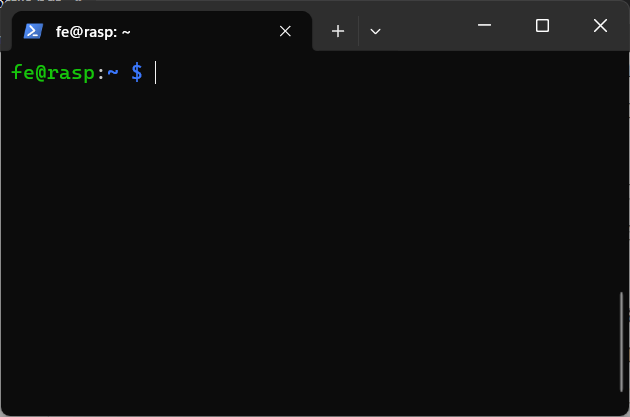
\includegraphics[width=0.8\linewidth]{prompt.png}
\caption{Exemplo de prompt de comando no Linux, exibindo \texttt{usuario@hostname:~\$}.}
\label{fig:prompt}
\end{figure}

\section{Fundamentos do Linux, Shell e Bash}

Agora que compreendemos o prompt de comando, vamos aprofundar nos conceitos fundamentais que permitem interagir com o sistema operacional de forma eficiente. Nesta seção, veremos o que é o Linux, o que é o shell, conheceremos o Bash e aprenderemos sobre os comandos integrados que formam a base do trabalho no terminal.

\subsection{O que é Linux}

Linux é um sistema operacional amplamente utilizado em servidores, computadores pessoais e sistemas embarcados. Em um sistema embarcado como o Orange Pi, ele permite controlar hardware, acessar dispositivos conectados, executar programas e organizar arquivos de forma estável e automatizável.

Tecnicamente, o Linux é o \textit{kernel}, isto é, o núcleo do sistema operacional. O kernel gerencia recursos como memória, processos, arquivos, rede e dispositivos físicos. Na prática, quando dizemos que uma máquina ``roda Linux'', geralmente estamos nos referindo a uma distribuição Linux, que combina o kernel com programas, bibliotecas, ferramentas de terminal e utilitários de administração.

Essa distinção é importante porque o usuário normalmente não interage diretamente com o kernel. A interação acontece por meio de programas, como o shell, que recebe comandos digitados no terminal e solicita ao sistema operacional que execute as ações correspondentes.

\begin{cmdbox}[Elementos Básicos de um Sistema Linux]
\begin{tabularx}{\linewidth}{@{}C >{\raggedright\arraybackslash}X >{\raggedright\arraybackslash}X@{}}
\toprule
\textbf{Elemento} & \textbf{Função} & \textbf{Exemplo} \\
\midrule
\texttt{kernel} & Núcleo que gerencia hardware e recursos do sistema & Linux \\
\texttt{distribuição} & Conjunto formado pelo kernel e ferramentas do sistema & Ubuntu, Debian, Armbian \\
\texttt{shell} & Programa que interpreta comandos do usuário & Bash \\
\texttt{terminal} & Interface usada para digitar comandos & Console, SSH, PowerShell \\
\bottomrule
\end{tabularx}
\end{cmdbox}

Em metrologia por imagem, essa estrutura é útil porque permite conectar câmeras, salvar imagens em diretórios organizados, executar scripts de captura e automatizar tarefas repetitivas. O acesso por SSH aproveita essa base: o aluno controla remotamente um sistema embarcado, mas os comandos são executados no Linux do próprio dispositivo.

\subsection{Sistema de Arquivos no Linux}

O Linux organiza arquivos e dispositivos em uma estrutura hierárquica de diretórios. O diretório principal é representado por \texttt{/}, chamado de raiz. A partir dele, aparecem diretórios como \texttt{/home}, \texttt{/etc}, \texttt{/dev}, \texttt{/var} e \texttt{/tmp}.

\begin{cmdbox}[Diretórios Comuns no Linux]
\begin{tabularx}{\linewidth}{@{}C >{\raggedright\arraybackslash}X >{\raggedright\arraybackslash}X@{}}
\toprule
\textbf{Diretório} & \textbf{Função} & \textbf{Exemplo de Uso} \\
\midrule
\texttt{/home} & Armazena arquivos dos usuários & \texttt{/home/usuario} \\
\texttt{/etc} & Contém arquivos de configuração do sistema & \texttt{/etc/hostname} \\
\texttt{/dev} & Representa dispositivos conectados ao sistema & \texttt{/dev/video0} \\
\texttt{/var} & Armazena dados variáveis, como logs & \texttt{/var/log} \\
\texttt{/tmp} & Guarda arquivos temporários & \texttt{/tmp/teste.txt} \\
\bottomrule
\end{tabularx}
\end{cmdbox}

Para esta aula, o mais importante é compreender que arquivos, diretórios e alguns dispositivos seguem a mesma lógica de navegação. Por exemplo, uma webcam pode aparecer como \texttt{/dev/video0}, enquanto imagens capturadas podem ser salvas em um diretório dentro de \texttt{/home/usuario}.

\subsection{O que é o Shell}

O shell é um programa que atua como interface entre o usuário e o \textit{kernel} do sistema operacional. Ele interpreta comandos digitados pelo usuário, executa programas e gerencia processos, permitindo interagir com o sistema de forma textual via linha de comando.

O termo ``shell'' vem do inglês e significa ``casca'' ou ``concha'', pois o shell é como uma camada externa que envolve o kernel (o núcleo do sistema operacional), protegendo-o e facilitando a comunicação com o usuário, assim como uma casca protege o interior de uma fruta ou ostra.
Essa hierarquia (usuário → shell → kernel → hardware) permite que comandos executados no shell resultem em ações diretas no hardware, como acessar uma câmera para captura de imagens, o que é essencial em aplicações de metrologia por imagem.

\subsection{O que é o Bash}

O Bash (Bourne Again Shell) é um dos shells mais populares e amplamente utilizados em sistemas Linux e Unix-like. Ele é uma evolução do shell Bourne (sh), oferecendo recursos avançados como histórico de comandos, autocompletar, scripting e personalização via variáveis de ambiente.

Como shell padrão em muitas distribuições Linux, o Bash facilita a interação com o sistema através de comandos de linha, sendo ideal para tarefas administrativas, automação de scripts e desenvolvimento de sistemas.

\textbf{Observação}: No Windows, o equivalente mais próximo ao Bash é o PowerShell, que oferece recursos similares de \textit{scripting}, automação e linha de comando, facilitando tarefas administrativas e desenvolvimento em contextos técnicos. Alternativamente, o CMD (\textit{Command Prompt}) é um shell mais básico no Windows, similar ao sh original, mas com funcionalidades limitadas em comparação ao Bash ou PowerShell.

\subsection{Comandos Builtin do Bash}

Os comandos builtin do Bash são aqueles integrados diretamente ao shell, executados sem a necessidade de iniciar um novo processo. Eles são essenciais para navegação e controle do ambiente, como \texttt{cd} (mudar diretório), \texttt{pwd} (mostrar diretório atual), \texttt{echo} (exibir texto), \texttt{.} e \texttt{source} (executar scripts no shell atual).

Para verificar se um comando é builtin, use \texttt{type comando} no terminal. Se for builtin, a saída indicará isso; caso contrário, mostrará o caminho do executável externo. Isso ajuda a entender a eficiência e o comportamento dos comandos no Bash.

\section{Comandos Práticos de Navegação e Manipulação}

Com a base teórica consolidada, vamos agora explorar os comandos práticos que são utilizados no dia a dia do trabalho com o terminal. Estes comandos são essenciais para organizar arquivos, configurar ambientes e preparar o sistema para tarefas de metrologia por imagem.

\subsection{Comandos de Navegação}

Os comandos de navegação permitem explorar e mover-se pelos diretórios do sistema de arquivos. O comando \texttt{pwd} mostra o diretório atual, \texttt{ls} lista arquivos e pastas, e \texttt{cd} muda para outro diretório.

Um símbolo importante na navegação é o $\sim$, que representa o diretório home do usuário. É o local padrão onde arquivos pessoais e configurações são armazenados. Por exemplo, para o usuário ``fe'', o caminho seria \texttt{/home/fe}. O $\sim$ é uma forma conveniente de se referir ao diretório home independentemente do nome do usuário, facilitando a navegação.

Exemplos práticos:

\begin{cmdbox}[Comandos de Navegação em Diretórios]
\begin{tabularx}{\linewidth}{@{}C >{\raggedright\arraybackslash}X >{\raggedright\arraybackslash}X@{}}
\toprule
\textbf{Comando} & \textbf{Função} & \textbf{Exemplo de Uso} \\
\midrule
pwd & Mostrar diretório atual & \texttt{pwd} $\rightarrow$ \texttt{/home/usuario} \\
ls & Listar arquivos no diretório & \texttt{ls /etc} \\
ls -l & Listar com detalhes (permissões, datas) & \texttt{ls -l /home} \\
ls -la & Listar todos incluindo ocultos & \texttt{ls -la \~{}} \\
cd & Mudar de diretório & \texttt{cd /home/usuario} \\
cd .. & Voltar um diretório acima & \texttt{cd ..} \\
cd \~{} & Ir para o diretório home & \texttt{cd \~{}} \\
cd - & Voltar ao diretório anterior & \texttt{cd -} \\
\bottomrule
\end{tabularx}
\end{cmdbox}

\subsection{Comandos de Manipulação de Arquivos e Pastas}

Os comandos de manipulação permitem criar, copiar, mover, renomear e remover arquivos e pastas. Exemplos incluem \texttt{mkdir} (criar pasta), \texttt{touch} (criar arquivo vazio), \texttt{cp} (copiar), \texttt{mv} (mover/renomear) e \texttt{rm} (remover).

Exemplos práticos com resultados esperados:

\begin{cmdbox}[Comandos de Manipulação de Arquivos e Pastas]
\begin{tabularx}{\linewidth}{@{}C >{\raggedright\arraybackslash}X >{\raggedright\arraybackslash}X@{}}
\toprule
\textbf{Comando} & \textbf{Função} & \textbf{Exemplo de Uso} \\
\midrule
mkdir & Criar diretório & \texttt{mkdir nova\_pasta} \\
touch & Criar arquivo vazio & \texttt{touch arquivo.txt} \\
cp & Copiar arquivo/diretório & \texttt{cp arquivo.txt copia.txt} \\
mv & Mover ou renomear & \texttt{mv arquivo.txt renomeado.txt} \\
rm & Remover arquivo & \texttt{rm copia.txt} \\
rm -r & Remover diretório recursivo & \texttt{rm -r nova\_pasta} \\
cat & Exibir conteúdo do arquivo & \texttt{cat arquivo.txt} \\
\bottomrule
\end{tabularx}
\end{cmdbox}

\vspace{0.3cm}

O comando \texttt{echo} é particularmente útil para exibir texto no terminal ou criar arquivos com conteúdo. Veja as principais formas de uso:

\begin{cmdbox}[Comandos de Redirecionamento e Echo]
\begin{tabularx}{\linewidth}{@{}C >{\raggedright\arraybackslash}X >{\raggedright\arraybackslash}X@{}}
\toprule
\textbf{Comando} & \textbf{Função} & \textbf{Exemplo de Uso} \\
\midrule
echo & Exibir texto no terminal & \texttt{echo "Olá Mundo"} \\
echo \$VAR & Exibir valor de variável & \texttt{echo \$HOME} \\
\texttt{>} & Redirecionar (sobrescrever) & \texttt{echo "texto" > arquivo.txt} \\
\texttt{>>} & Redirecionar (anexar) & \texttt{echo "mais" >> arquivo.txt} \\
\bottomrule
\end{tabularx}
\end{cmdbox}

\subsection{Redirecionamento de Fluxo e Pipes}

Além dos redirecionamentos de entrada e saída com \texttt{>} e \texttt{>>}, o Bash oferece o operador pipe (\texttt{|}), que conecta a saída de um comando à entrada de outro. Essa é uma das funcionalidades mais poderosas do shell, permitindo construir pipelines complexos para processamento de dados.

Por exemplo, é possível listar arquivos, filtrar resultados e contar linhas em uma única linha de comando. Em metrologia por imagem, pipes são úteis para encadear comandos de processamento, como converter imagens, extrair metadados e gerar estatísticas sequencialmente.

\begin{cmdbox}[Operador Pipe (\texttt{|})]
\begin{tabularx}{\linewidth}{@{}C >{\raggedright\arraybackslash}X >{\raggedright\arraybackslash}X@{}}
\toprule
\textbf{Comando} & \textbf{Função} & \textbf{Exemplo de Uso} \\
\midrule
\texttt{|} & Conectar saída de um comando à entrada de outro & \texttt{ls -l | grep ".txt"} \\
\texttt{grep} & Filtrar linhas por padrão de texto & \texttt{cat log.txt | grep "erro"} \\
\texttt{sort} & Ordenar linhas & \texttt{ls | sort} \\
\texttt{wc} & Contar linhas, palavras e caracteres & \texttt{ls -l | wc -l} \\
\texttt{head} & Exibir primeiras linhas & \texttt{ls -l | head -n 5} \\
\texttt{tail} & Exibir últimas linhas & \texttt{cat log.txt | tail -n 10} \\
\texttt{less} & Visualizar saída longa interativamente & \texttt{cat log.txt | less} \\
\bottomrule
\end{tabularx}
\end{cmdbox}

\subsection{Variáveis de Ambiente}

As variáveis de ambiente são valores nomeados que influenciam o comportamento de programas e do próprio shell. Elas são fundamentais para configurar caminhos de execução, diretórios padrão e preferências do sistema.

No Bash, variáveis são acessadas com o prefixo \texttt{\$}. A variável \texttt{PATH}, por exemplo, define os diretórios onde o shell procura por executáveis. Em projetos de metrologia, variáveis podem apontar para diretórios de imagens, configurações de câmera ou caminhos de bibliotecas de processamento.

\begin{cmdbox}[Variáveis de Ambiente Comuns]
\begin{tabularx}{\linewidth}{@{}C >{\raggedright\arraybackslash}X >{\raggedright\arraybackslash}X@{}}
\toprule
\textbf{Variável} & \textbf{Função} & \textbf{Exemplo de Uso} \\
\midrule
\texttt{\$HOME} & Diretório home do usuário & \texttt{echo \$HOME} \\
\texttt{\$PATH} & Caminhos de busca de executáveis & \texttt{echo \$PATH} \\
\texttt{\$USER} & Nome do usuário atual & \texttt{echo \$USER} \\
\texttt{\$PWD} & Diretório de trabalho atual & \texttt{echo \$PWD} \\
\texttt{export} & Definir variável de ambiente & \texttt{export CAM\_DIR=/home/fe/imagens} \\
\bottomrule
\end{tabularx}
\end{cmdbox}

\subsection{Permissões de Arquivos}

O Linux utiliza um sistema de permissões para controlar acesso a arquivos e diretórios. Cada arquivo possui permissões de leitura (\texttt{r}), escrita (\texttt{w}) e execução (\texttt{x}) para três categorias: proprietário, grupo e outros.

O comando \texttt{chmod} (change mode) altera as permissões, enquanto \texttt{chown} (change owner) altera o proprietário do arquivo. Em ambientes de metrologia, é comum configurar permissões para que múltiplos usuários ou processos possam acessar imagens e dados coletados.

\begin{cmdbox}[Gerenciamento de Permissões]
\begin{tabularx}{\linewidth}{@{}C >{\raggedright\arraybackslash}X >{\raggedright\arraybackslash}X@{}}
\toprule
\textbf{Comando} & \textbf{Função} & \textbf{Exemplo de Uso} \\
\midrule
\texttt{ls -l} & Visualizar permissões & \texttt{ls -l arquivo.txt} \\
\texttt{chmod +x} & Adicionar permissão de execução & \texttt{chmod +x script.sh} \\
\texttt{chmod 755} & Definir permissões numericamente & \texttt{chmod 755 diretorio} \\
\texttt{chmod 644} & Arquivo: leitura para todos & \texttt{chmod 644 imagem.png} \\
\texttt{chown} & Alterar proprietário & \texttt{chown usuario arquivo.txt} \\
\bottomrule
\end{tabularx}
\end{cmdbox}

\subsection{Processos em Segundo Plano}

Em tarefas de metrologia por imagem, como capturas contínuas ou processamentos longos, é comum executar comandos em segundo plano. O Bash oferece mecanismos simples para gerenciar processos sem bloquear o terminal.

\begin{cmdbox}[Gerenciamento de Processos]
\begin{tabularx}{\linewidth}{@{}C >{\raggedright\arraybackslash}X >{\raggedright\arraybackslash}X@{}}
\toprule
\textbf{Comando} & \textbf{Função} & \textbf{Exemplo de Uso} \\
\midrule
\texttt{\&} & Executar em segundo plano & \texttt{python captura.py \&} \\
\texttt{jobs} & Listar processos em segundo plano & \texttt{jobs} \\
\texttt{fg} & Trazer processo para primeiro plano & \texttt{fg \%1} \\
\texttt{Ctrl+C} & Interromper processo em execução & \textit{(pressione no terminal)} \\
\texttt{nohup} & Executar sem interromper ao sair & \texttt{nohup processo.sh \&} \\
\bottomrule
\end{tabularx}
\end{cmdbox}

\subsection{Loops e Decisões em Scripts Bash}

O Bash permite a criação de scripts para automatizar tarefas repetitivas e tomar decisões com base em condições. Essa funcionalidade é essencial em projetos de metrologia por imagem, onde é comum processar centenas de imagens, verificar a existência de arquivos de configuração ou executar rotinas de captura sequenciais.

Os loops \texttt{for} e \texttt{while} permitem repetir operações sobre listas de arquivos ou aguardar condições específicas. Já as estruturas condicionais \texttt{if/else} possibilitam executar comandos diferentes dependendo do resultado de testes, como verificar se um arquivo existe ou se um comando foi executado com sucesso.

\begin{cmdbox}[Estruturas de Loop]
\begin{tabularx}{\linewidth}{@{}C >{\raggedright\arraybackslash}X >{\raggedright\arraybackslash}X@{}}
\toprule
\textbf{Estrutura} & \textbf{Função} & \textbf{Exemplo de Uso} \\
\midrule
\texttt{for} & Iterar sobre uma lista & \texttt{for f in *.png; do echo \$f; done} \\
\texttt{for seq} & Iterar com sequência numérica & \texttt{for i in \{1..10\}; echo \$i; done} \\
\texttt{while} & Repetir enquanto condição verdadeira & \texttt{while [ -f lock ]; do sleep 1; done} \\
\texttt{break} & Sair do loop antecipadamente & \texttt{if [ \$i -eq 5 ]; then break; fi} \\
\texttt{continue} & Pular para próxima iteração & \texttt{if [ ! -f \$f ]; then continue; fi} \\
\bottomrule
\end{tabularx}
\end{cmdbox}

\begin{cmdbox}[Estruturas Condicionais]
\begin{tabularx}{\linewidth}{@{}C >{\raggedright\arraybackslash}X >{\raggedright\arraybackslash}X@{}}
\toprule
\textbf{Estrutura} & \textbf{Função} & \textbf{Exemplo de Uso} \\
\midrule
\texttt{if/then} & Executar se condição verdadeira & \texttt{if [ -f config.txt ]; then echo "OK"; fi} \\
\texttt{if/else} & Alternativa se falso & \texttt{if [ -f img.png ]; then process; else echo "Falha"; fi} \\
\texttt{elif} & Múltiplas condições & \texttt{if [ \$r -eq 0 ]; then ... elif [ \$r -eq 1 ]; then ... fi} \\
\texttt{[ -f ]} & Testar se arquivo existe & \texttt{[ -f /home/fe/dados.csv ]} \\
\texttt{[ -d ]} & Testar se diretório existe & \texttt{[ -d /home/fe/imagens ]} \\
\texttt{[ -s ]} & Testar se arquivo não está vazio & \texttt{[ -s log.txt ]} \\
\bottomrule
\end{tabularx}
\end{cmdbox}

Um exemplo prático de script que processa todas as imagens PNG em um diretório:

\begin{cmdbox}[Exemplo de Script de Processamento]
\begin{tabularx}{\linewidth}{@{}C >{\raggedright\arraybackslash}X@{}}
\toprule
\textbf{Linha} & \textbf{Código} \\
\midrule
1 & \texttt{\#!/bin/bash} \\
2 & \texttt{for img in *.png; do} \\
3 & \texttt{\ \ \ echo "Processando: \$img"} \\
4 & \texttt{\ \ \ if [ -s "\$img" ]; then} \\
5 & \texttt{\ \ \ \ \ \ python processar.py "\$img"} \\
6 & \texttt{\ \ \ else} \\
7 & \texttt{\ \ \ \ \ \ echo "Arquivo vazio: \$img"} \\
8 & \texttt{\ \ \ fi} \\
9 & \texttt{done} \\
\bottomrule
\end{tabularx}
\end{cmdbox}

Neste exemplo, o script itera sobre todas as imagens PNG, verifica se cada arquivo possui conteúdo (não está vazio) e, em caso positivo, executa um script Python de processamento. Caso o arquivo esteja vazio, exibe uma mensagem de aviso.

\section{Escrita de Scripts Bash (Automação)}

Nesta seção, vamos reunir os conceitos apresentados anteriormente para construir pequenos scripts Bash. Um script é um arquivo de texto com comandos organizados em sequência. Em vez de digitar cada comando manualmente no terminal, o usuário escreve a rotina uma vez e depois executa o arquivo sempre que precisar repetir a tarefa.

Em metrologia por imagem, essa prática é importante porque ajuda a reduzir variações introduzidas pelo operador. A mesma sequência de comandos pode ser usada para preparar diretórios, capturar imagens, registrar nomes de arquivos, processar dados e repetir medições de forma mais padronizada.

\subsection{O que é um Script Bash}

Um script Bash contém comandos que poderiam ser executados diretamente no terminal. A diferença é que, no script, esses comandos ficam salvos em um arquivo e são executados de forma automática pelo shell.

Isso permite transformar uma tarefa manual em uma rotina reprodutível. Por exemplo, em vez de lembrar todos os comandos necessários para capturar e organizar imagens, podemos registrar esses passos em um arquivo como \texttt{captura.sh}.

\subsection{Estrutura Básica de um Script}

Um script Bash normalmente começa com a linha \texttt{\#!/bin/bash}, chamada de \textit{shebang}. Ela informa ao sistema que o arquivo deve ser interpretado pelo Bash.

\begin{cmdbox}[Script Bash Simples]
\begin{tabularx}{\linewidth}{@{}C >{\raggedright\arraybackslash}X@{}}
\toprule
\textbf{Linha} & \textbf{Código} \\
\midrule
1 & \texttt{\#!/bin/bash} \\
2 & \texttt{echo "Olá, mundo!"} \\
\bottomrule
\end{tabularx}
\end{cmdbox}

Depois de criar o arquivo, é necessário adicionar permissão de execução e chamá-lo pelo terminal.

\begin{cmdbox}[Executando um Script]
\begin{tabularx}{\linewidth}{@{}C >{\raggedright\arraybackslash}X >{\raggedright\arraybackslash}X@{}}
\toprule
\textbf{Comando} & \textbf{Função} & \textbf{Exemplo de Uso} \\
\midrule
\texttt{chmod +x} & Tornar o script executável & \texttt{chmod +x script.sh} \\
\texttt{./script.sh} & Executar o script no diretório atual & \texttt{./script.sh} \\
\bottomrule
\end{tabularx}
\end{cmdbox}

O prefixo \texttt{./} indica que o arquivo está no diretório atual. Sem esse prefixo, o shell procuraria o comando apenas nos diretórios definidos na variável \texttt{PATH}.

\subsection{Uso de Parâmetros}

Scripts também podem receber informações pela linha de comando. Esses valores são chamados de parâmetros ou argumentos. No Bash, \texttt{\$1} representa o primeiro parâmetro, \texttt{\$2} representa o segundo, e assim por diante.

\begin{cmdbox}[Script com Parâmetro]
\begin{tabularx}{\linewidth}{@{}C >{\raggedright\arraybackslash}X@{}}
\toprule
\textbf{Linha} & \textbf{Código} \\
\midrule
1 & \texttt{\#!/bin/bash} \\
2 & \texttt{echo "Arquivo recebido: \$1"} \\
\bottomrule
\end{tabularx}
\end{cmdbox}

\begin{cmdbox}[Execução com Parâmetro]
\begin{tabularx}{\linewidth}{@{}C >{\raggedright\arraybackslash}X >{\raggedright\arraybackslash}X@{}}
\toprule
\textbf{Comando} & \textbf{Função} & \textbf{Exemplo de Uso} \\
\midrule
\texttt{./script.sh imagem.png} & Executar o script passando um arquivo & \texttt{./script.sh imagem.png} \\
\texttt{\$1} & Acessar o primeiro parâmetro dentro do script & \texttt{imagem.png} \\
\bottomrule
\end{tabularx}
\end{cmdbox}

Esse recurso é útil quando o mesmo script deve ser aplicado a arquivos diferentes, como imagens capturadas em momentos distintos.

\subsection{Automação com Loops}

Loops permitem repetir comandos automaticamente. Um caso comum é percorrer todos os arquivos de imagem de um diretório e executar uma ação para cada arquivo encontrado.

\begin{cmdbox}[Processamento de Imagens com \texttt{for}]
\begin{tabularx}{\linewidth}{@{}C >{\raggedright\arraybackslash}X@{}}
\toprule
\textbf{Linha} & \textbf{Código} \\
\midrule
1 & \texttt{\#!/bin/bash} \\
2 & \texttt{for img in *.png; do} \\
3 & \texttt{\ \ \ echo "Processando: \$img"} \\
4 & \texttt{\ \ \ python processar.py "\$img"} \\
5 & \texttt{done} \\
\bottomrule
\end{tabularx}
\end{cmdbox}

Neste exemplo, o Bash procura arquivos com extensão \texttt{.png}. Para cada arquivo encontrado, o nome é armazenado temporariamente na variável \texttt{img}, que pode ser usada pelos comandos dentro do loop.

\subsection{Tomada de Decisão com Condicionais}

Estruturas condicionais permitem executar comandos apenas quando uma condição é satisfeita. Isso é útil para evitar erros, como tentar processar um arquivo que não existe ou que está vazio.

\begin{cmdbox}[Verificação de Arquivo com \texttt{if}]
\begin{tabularx}{\linewidth}{@{}C >{\raggedright\arraybackslash}X@{}}
\toprule
\textbf{Linha} & \textbf{Código} \\
\midrule
1 & \texttt{\#!/bin/bash} \\
2 & \texttt{if [ -f "config.txt" ]; then} \\
3 & \texttt{\ \ \ echo "Arquivo encontrado"} \\
4 & \texttt{else} \\
5 & \texttt{\ \ \ echo "Arquivo não encontrado"} \\
6 & \texttt{fi} \\
\bottomrule
\end{tabularx}
\end{cmdbox}

O teste \texttt{[ -f "config.txt" ]} verifica a existência do arquivo. Se a condição for verdadeira, o primeiro bloco é executado; caso contrário, o bloco após \texttt{else} é executado.

\subsection{Exemplo Aplicado: Captura Periódica de Imagens}

Em uma rotina de aquisição, o script pode capturar imagens em intervalos regulares. O exemplo abaixo cria um nome de arquivo com data e hora, captura uma imagem e aguarda 60 segundos antes da próxima captura.

\begin{cmdbox}[Captura Periódica de Imagens]
\begin{tabularx}{\linewidth}{@{}C >{\raggedright\arraybackslash}X@{}}
\toprule
\textbf{Linha} & \textbf{Código} \\
\midrule
1 & \texttt{\#!/bin/bash} \\
2 & \texttt{while true; do} \\
3 & \texttt{\ \ \ nome="img\_\$(date +\%Y\%m\%d\_\%H\%M\%S).jpg"} \\
4 & \texttt{\ \ \ echo "Capturando: \$nome"} \\
5 & \texttt{\ \ \ fswebcam "\$nome"} \\
6 & \texttt{\ \ \ sleep 60} \\
7 & \texttt{done} \\
\bottomrule
\end{tabularx}
\end{cmdbox}

\begin{cmdbox}[Elementos do Script de Captura]
\begin{tabularx}{\linewidth}{@{}C >{\raggedright\arraybackslash}X >{\raggedright\arraybackslash}X@{}}
\toprule
\textbf{Elemento} & \textbf{Função} & \textbf{Exemplo de Uso} \\
\midrule
\texttt{while true} & Repetir continuamente & \texttt{while true; do ... done} \\
\texttt{date} & Gerar data e hora para o nome do arquivo & \texttt{date +\%Y\%m\%d\_\%H\%M\%S} \\
\texttt{fswebcam} & Capturar imagem da webcam & \texttt{fswebcam imagem.jpg} \\
\texttt{sleep} & Aguardar antes da próxima repetição & \texttt{sleep 60} \\
\bottomrule
\end{tabularx}
\end{cmdbox}

Esse tipo de script ainda depende de um terminal aberto para continuar rodando. Nas próximas etapas do curso, a automação poderá ser transferida para o \texttt{systemd}, permitindo que a captura seja iniciada e controlada pelo próprio sistema.

\subsection{Integração com Pipes}

Scripts também podem usar pipes para combinar comandos. Isso facilita a criação de pequenos fluxos de processamento sem precisar salvar resultados intermediários em arquivos.

\begin{cmdbox}[Uso de Pipe em Script]
\begin{tabularx}{\linewidth}{@{}C >{\raggedright\arraybackslash}X >{\raggedright\arraybackslash}X@{}}
\toprule
\textbf{Comando} & \textbf{Função} & \textbf{Exemplo de Uso} \\
\midrule
\texttt{ls *.png} & Listar imagens PNG & \texttt{ls *.png} \\
\texttt{sort} & Ordenar a lista de arquivos & \texttt{ls *.png | sort} \\
\texttt{head -n 5} & Exibir apenas os cinco primeiros itens & \texttt{ls *.png | sort | head -n 5} \\
\bottomrule
\end{tabularx}
\end{cmdbox}

No exemplo, a saída de \texttt{ls *.png} é enviada para \texttt{sort}, e a saída ordenada é enviada para \texttt{head -n 5}. Assim, cada comando executa uma parte simples da tarefa.

\subsection{Considerações Finais}

A escrita de scripts Bash permite transformar comandos isolados em rotinas claras, repetíveis e fáceis de registrar. Em experimentos de metrologia por imagem, isso contribui para maior organização dos dados e maior consistência na execução das etapas de aquisição e processamento.

Com os conceitos desta seção, já é possível criar scripts simples para automatizar tarefas locais. Esse conhecimento servirá de base para scripts de captura em Python e para a automação com \texttt{systemd} nas próximas aulas.

\section{Conclusão}

Neste módulo, vimos os conceitos e comandos básicos necessários para acessar e operar um sistema Linux remotamente. O SSH permite entrar no dispositivo pela rede; o terminal fornece a interface de trabalho; o shell interpreta os comandos; e o Bash permite tanto a execução manual quanto a criação de scripts simples.

Esses recursos formam a base para uma rotina de metrologia por imagem mais organizada e reprodutível. A partir deles, é possível navegar por diretórios, manipular arquivos, verificar permissões, usar variáveis, encadear comandos com pipes e automatizar pequenas tarefas de captura ou processamento.

Nas próximas aulas, essa base será usada para construir scripts de captura em Python e, posteriormente, automatizar sua execução com \texttt{systemd}. Assim, o processo deixa de depender de ações manuais repetidas e passa a se aproximar de um sistema de aquisição contínuo, controlado e mais confiável.

\end{document}
